\chapter[SCP-046 “掠食性”冬青树丛]{
    SCP-046 "Predatory" Holly Bush\\
    SCP-046 “掠食性”冬青树丛
}

\label{chap:SCP-046}

\begin{figure}[H]
    \centering
    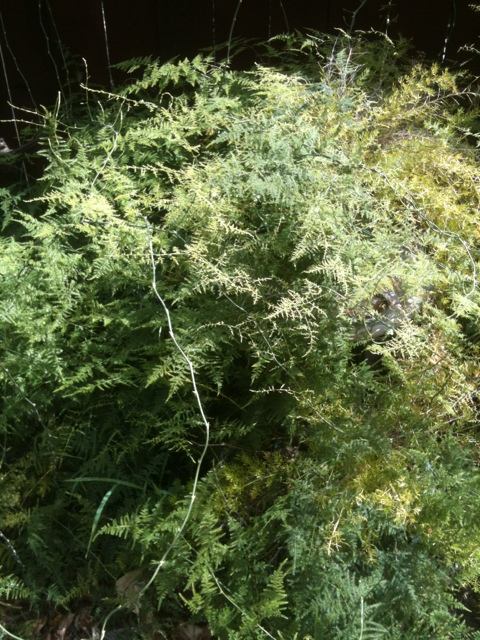
\includegraphics[width=0.5\linewidth]{images/SCP.046.jpg}
    \caption*{SCP-046的独立分枝,主要由耳蕨属成员组成。}
\end{figure}

\bb{项目编号:}SCP-046

\bb{项目分类:}Euclid

\bb{特殊收容措施:}SCP-046周边的土地已经被买下并被包括围栏、路障和致命陷阱等的多层安全措施包围起来;应在显眼处设立数个将该区域标注为私有财产的标志。该区域应随时严加守卫以防止平民接触SCP-046。所有在周边或在SCP-046半径50km范围内工作的人员应接受细致的体检以确保未患有任何可能危及生命的疾病;此外,应增加精神健康检测的次数以确保没有倾向或可能倾向自残或自毁的人员进入半径50km范围内。任何受伤人员应被转移至SCP-046周边50km地带以外的医院。SCP-046周边的所有植被应被摧毁,所有尝试接触SCP-046的动物应在到达其外部边界之前被处决并销毁。

任何显示出对SCP-046或对进入SCP-046附近地区有异常兴趣的人员应接受上文详述的体检。对收容措施的任何调整在添加进该收容文档前应由O5指挥部批准。任何没有被适当地授权而尝试修改该文档的人员将被降级并重新指派工作。

\bb{描述:}SCP-046是位于(美国)肯塔基州西南部的一团掠食性植物。SCP-046由两部分组成。SCP-046-1是一大团植物,主要由当地原产植物构成,包括白栎、欧洲冬青和贯月忍冬,但也能找到其它种植物的分枝。SCP-046-2是从SCP-046-1基部向其附近延伸的土地,区域大致呈圆形,半径二十米。该区域是SCP-046的主要摄食区。SCP-046能够利用幻觉吸引半径50km范围内的猎物;每一次人员转移均应将人员带到该半径之外以消除SCP-046的影响。

为可能危及生命的身体损伤或疾病,或者导致自毁倾向的精神错乱所苦的动物(包括人类),会感到一阵来到SCP-046-2并面朝SCP-046-1趴下的强烈冲动。以这种姿势趴着的个体很快被一种异常强大的腐生性微生物和机会性感染\footnote{\bb{译注:} 机会性感染:对免疫系统受损的人有害的感染。}联合体所袭击,包括数种已知能引发坏死性筋膜炎\footnote{\bb{译注:} 坏死性筋膜炎(Necrotizing fasciitis),又称“食肉细菌感染”,是一种由细菌入侵皮下组织和筋膜引起的急性坏死性软组织感染。这种疾病在临床上较为少见,但发病急,进展较快,破坏力强,病死率较高,并会造成严重的残疾。临床表现为沿深浅筋膜播散的感染,在累及血管内形成血栓,引起相应皮下组织、皮肤和筋膜的坏死。可发生在全身各个部位,四肢较为多见,尤其是下肢;其次是会阴、颈部、面部、腹壁和背臀部等。严重时受感染部位的内部组织完全暴露在体外,坏死部分形成凹陷}的耐甲氧西林\ii{金黄色葡萄球菌}(MRSA),也被称为“食肉细菌”;一种使猎物中毒并导致瘫痪的与\ii{黑葡萄穗霉},或称“黑霉”相似的真菌的孢子;最后,在摄食的最终阶段,从SCP-046-1内部出现的几种之前尚未知晓的昆虫(将猎物)吃光。SCP-046似乎通过对受影响的个体,尤其是像人类这样的大型哺乳动物的完全消化来获取营养。不清楚SCP-046是否有能力成长;有鉴于此,应采取一切措施以确保SCP-046没有猎物,直到获得更多关于其能力的信息。这些努力应包括在个体到达SCP-046前进行处决并在(与SCP-046)无关的地点处理尸体。

\bb{附录046-A} 因为某些人员在对SCP-046的反应中表现出的异常效果,对由关于SCP-046的知识引发的潜在的模因效应的调查正在进行。文档046-07仅允许4级及以上人员查看。

\tred{文档046-07}

\tred{隐藏}

\begin{figure}[H]
    \centering
    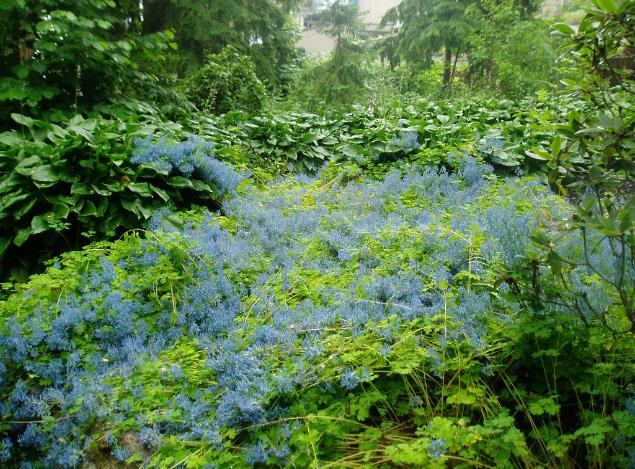
\includegraphics[width=0.5\linewidth]{images/SCP.046.2.jpg}
    \caption*{SCP-046的大型分枝,主要由蓝色紫堇组成。}
\end{figure}

\bb{项目编号:}SCP-046

\bb{项目分类:}Safe

\bb{特殊收容措施:}SCP-046周边的土地应被封锁、标注为私有财产并由多层围栏环绕。该区域应由至少十名守卫保护,但只需要最少的武装。虽然关于SCP-046效应的知识不应被大范围传播,但可允许患有危及生命的疾病的人员在自毁倾向心理检查后进入SCP-046-2。类似地,被选中处决的D级人员可被有效地暴露于SCP-046-2以使过程更便利。由于对基金会安保缺乏威胁性,可以允许未被基金会雇佣的个人接触SCP-046,但基金会的接触需求是第一位的。

\bb{描述:}SCP-046由两部分组成。SCP-046-1是一个直径5m,高30m的圆柱形区域,内含数种植物,包括白栎、欧洲冬青和贯月忍冬(肯塔基忍冬),但也能找到其它种植物的分枝。未从这些植物的分子构成上检测出反常特征。SCP-046-2是从SCP-046-1向周围延伸约二十米的一片长草的空地。

SCP-046的异常效应主要影响受慢性或使人衰弱的疾病及伤痛威胁的动物,包括人类。这类个体经常来到SCP-046;这种类型的人类反映感到一种去SCP-046所在地的冲动,常说这个地点“在梦里见过”。心理评估一致表明这些个体之前既不了解基金会也不清楚SCP-046的特性。感受到这种冲动的个体都报告称当时处在SCP-046半径50km范围内;据信这是对象的吸引范围的外部边界。

来到SCP-046的个体一致描述了一个梦,梦中他们在SCP-046-1周围躺下休息。进入SCP-046-2的瞬间,受长期疼痛或精神创伤困扰的个体会声称他们的症状逐渐减弱,同时感到平静、放松和极度的愉快与兴奋。在SCP-046-1面前躺下的个体将开始被数根与也被称为“百慕大草”的狗牙根草的纤匐枝相似的藤条覆盖,之后狗牙根草以肉眼可见的速度长满其全身。SCP-046没有吸引人的性质,其效果只会在自愿受影响的个体身上显现。

被暴露于SCP-046的个体将保持语言能力直到他们被身体上的草掩盖得再也无法被看见。所有被暴露于SCP-046的影响下的个体描述了一种平静安详的感觉以及能够愉快地死去的幸福感。SCP-046看来能在两小时内完全分解受影响的个体,不清楚是否将分解后的组织作为食物来源。

\bb{附录046-1:}O5指挥部指示,SCP-046应被重分级为Euclid,最初的收容文档应被重写以展示SCP-046的掠食天性。任何提及“自愿个体”的部分都应被移除。描述应被重写以强调SCP-046不稳定和致命的本质及其潜在威胁。

\bb{附录046-2:}\ii{没有一点证据证明SCP-046是“掠食性”的或者有任何伤害不愿将自己暴露于SCP-046影响之下的任何生物的欲望。建议重新启用原收容措施,继续对SCP-046的自愿访问。只要被暴露在SCP-046面前,没有人能够突破基金会的安保;基于此,没有理由拒绝给予受苦的个体解脱的机会。同样,没有理由让这个实体显得比实际上更有敌意,这也适用于那种将基金会保管的每一个对象描绘成危险品的欲望。有些东西只是因为它们很奇怪才必须被收容。}——Edward Carter博士,SCP-046研究主管

\bb{附录046-3:}SCP-046的主要研究员Carter博士应被调离其岗位并重新指派到另一个项目。在O5指挥部命令下附录046-1继续生效。
